\documentclass{slides}
\title{Drivetrain Update Flow}
\author{Natan Jurca}
\date{September 2025}

\usepackage{tikz}
\usepackage[top=1cm, bottom=1cm, right=1cm, left=1cm]{geometry}
\usetikzlibrary{shapes.geometric, arrows}
\usetikzlibrary{positioning}

\tikzstyle{startstop} = [rectangle, rounded corners, minimum width=3cm, minimum height=1cm,text centered, draw=black, fill=red!30]
\tikzstyle{io} = [trapezium, trapezium left angle=70, trapezium right angle=110, minimum width=3cm, minimum height=1cm, text centered, draw=black]
\tikzstyle{process} = [rectangle, minimum width=3cm, minimum height=1cm, text centered, draw=black]
\tikzstyle{decision} = [diamond, aspect=2, minimum width=3cm, minimum height=1cm, text centered, draw=black]
\tikzstyle{big_decision} = [diamond, aspect=4, minimum width=3cm, minimum height=1cm, text centered, draw=black]
\tikzstyle{arrow} = [thick,->,>=latex]

\begin{document}
\resizebox{\textwidth}{\textheight}{%
	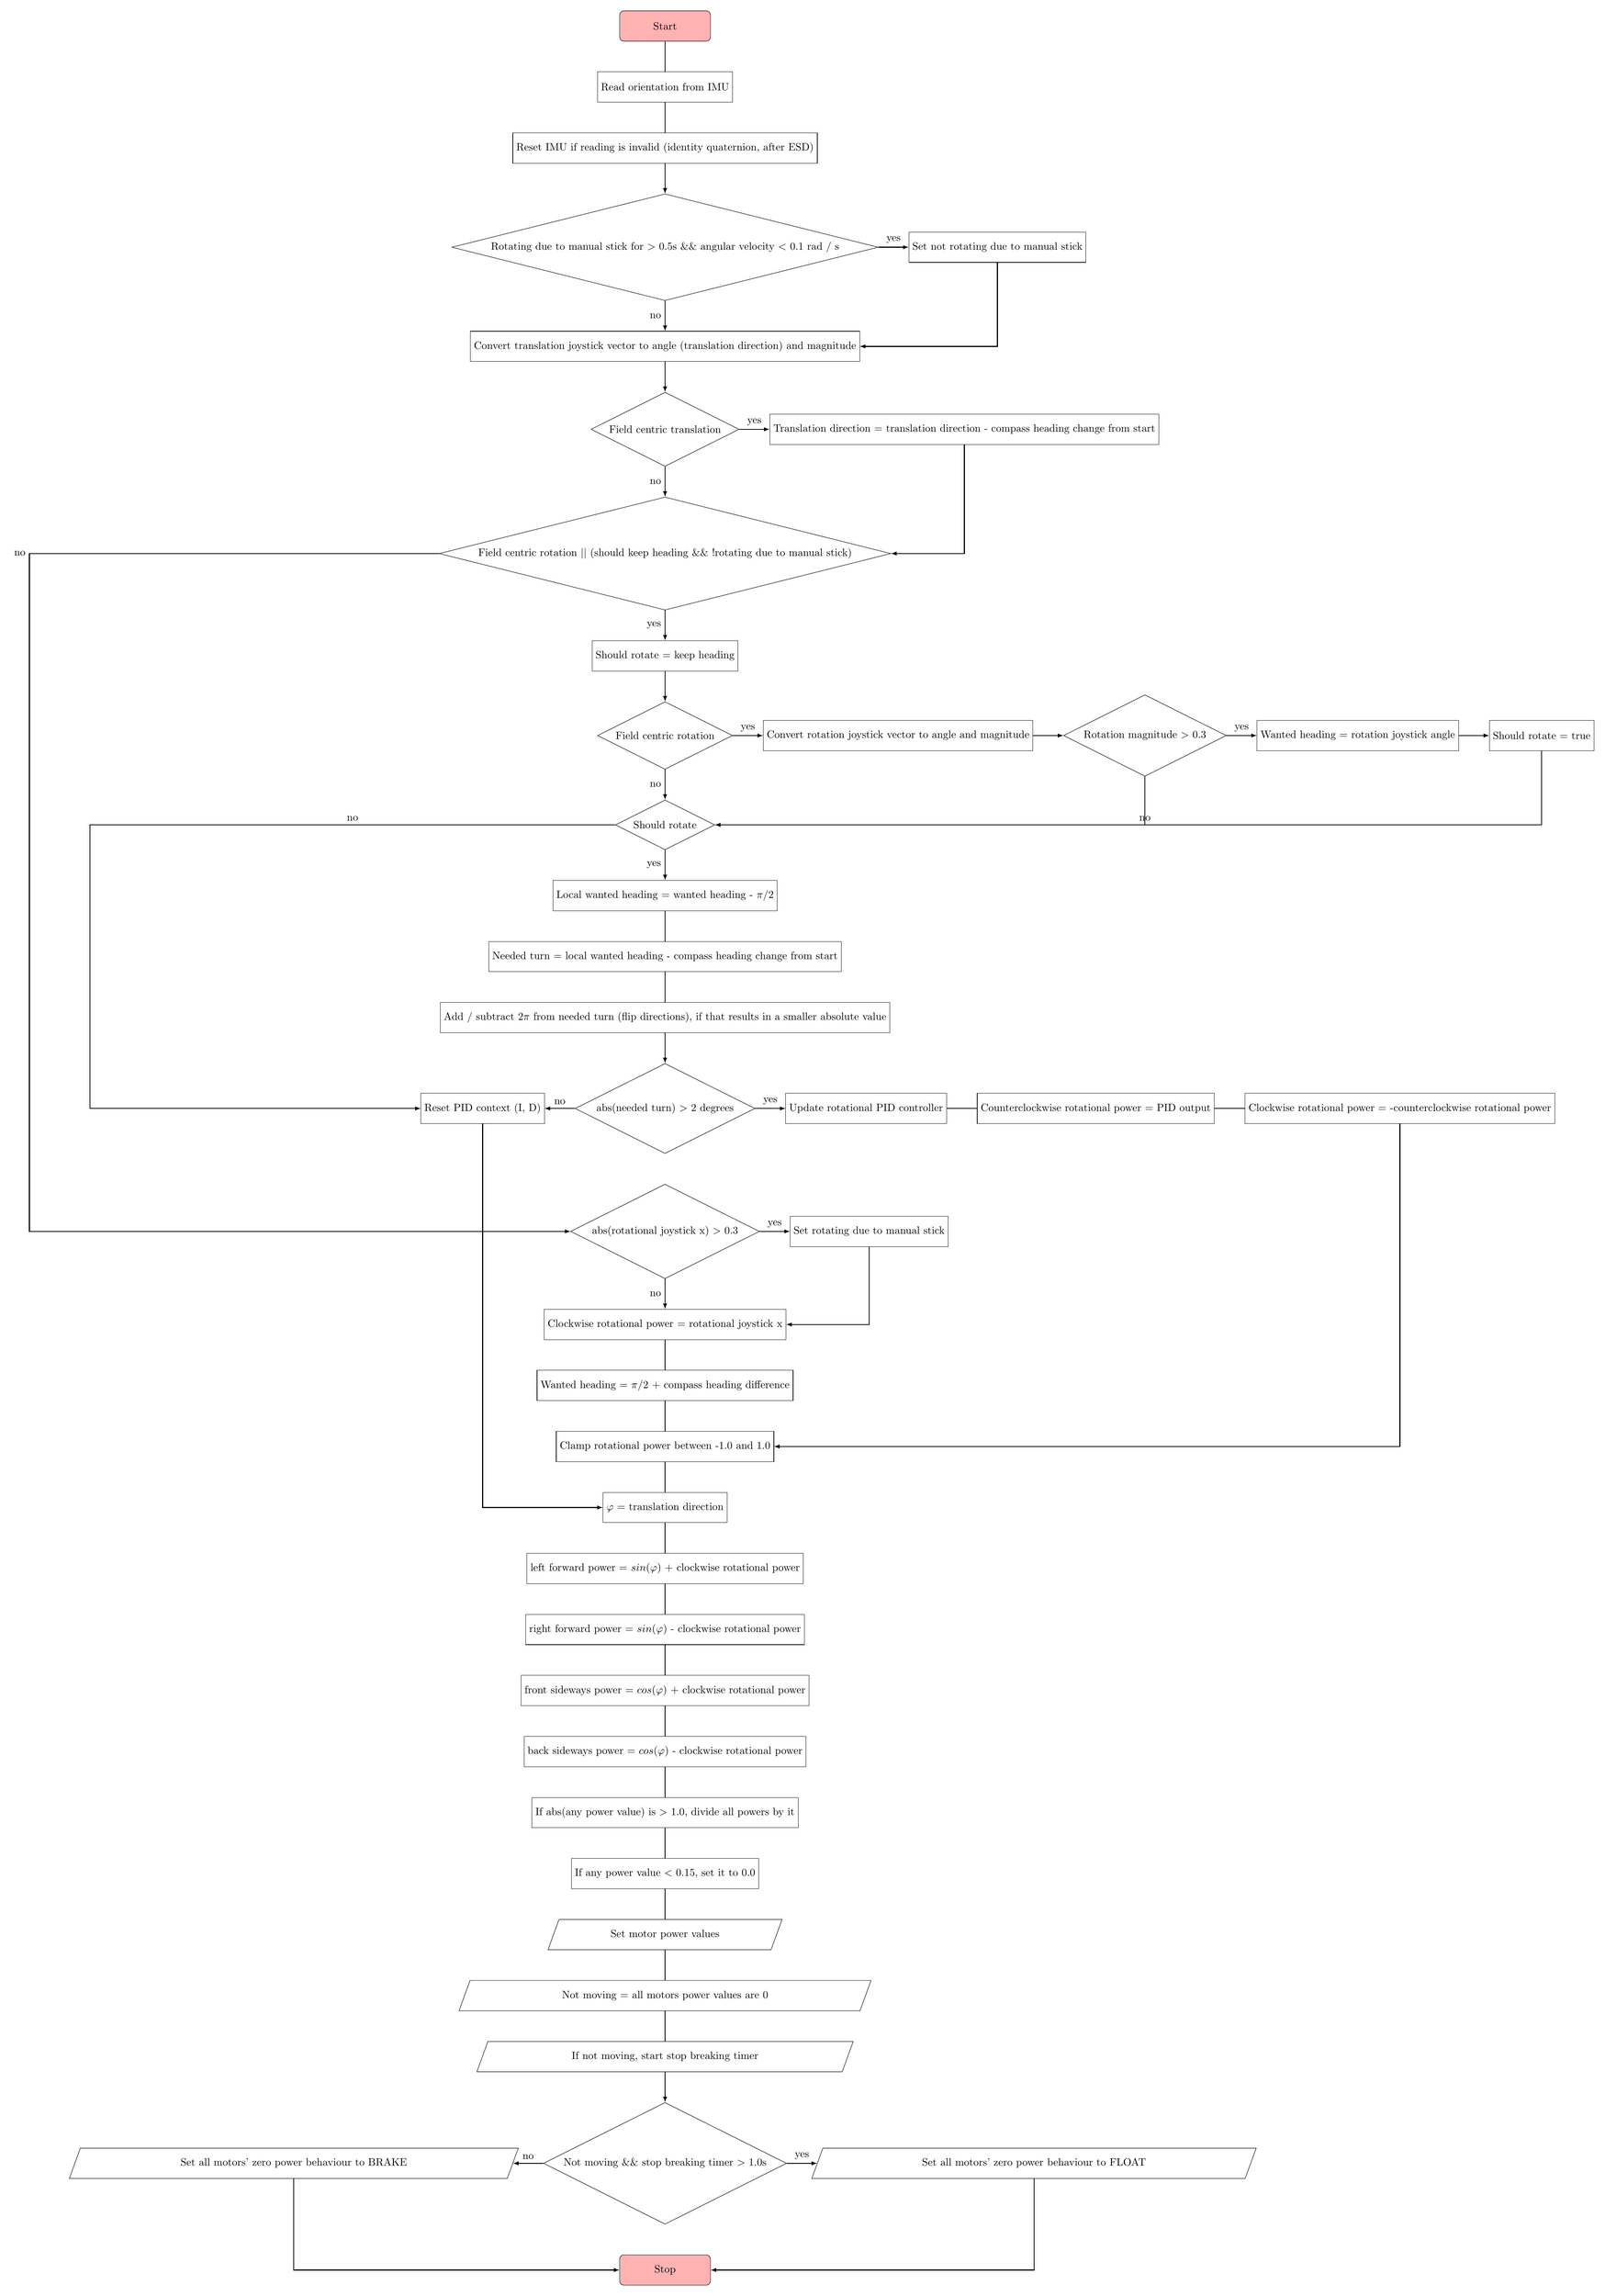
\begin{tikzpicture}[node distance=1cm]
		\node at (0, 0) (start) [startstop] {Start};
		\node (read_from_imu) [process, below=of start] {Read orientation from IMU};
		\node (fix_imu) [process, below=of read_from_imu] {Reset IMU if reading is invalid (identity quaternion, after ESD)};

		\node (stop_manual_rotation_if) [big_decision, below=of fix_imu] {Rotating due to manual stick for $>$ 0.5s \&\& angular velocity $<$ 0.1 rad / s};

		\node (not_rotating_due_to_manual_stick) [process, right=of stop_manual_rotation_if] {Set not rotating due to manual stick};

		\node (get_magnitude_and_phi_for) [process, below=of stop_manual_rotation_if] {Convert translation joystick vector to angle (translation direction) and magnitude};

		\node (field_centric_translation_if) [decision, below=of get_magnitude_and_phi_for] {Field centric translation};

		\node (compensate_for_heading_difference) [process, right=of field_centric_translation_if] {Translation direction = translation direction - compass heading change from start};

		\node (field_centric_rotation_if) [big_decision, below=of field_centric_translation_if] {Field centric rotation $||$ (should keep heading \&\& !rotating due to manual stick)};

		\node (should_rotate) [process, below=of field_centric_rotation_if] {Should rotate = keep heading};

		\node (if_field_centric_rotation) [decision, below=of should_rotate] {Field centric rotation};
		\node (get_magnitude_and_phi_for_rotation) [process, right=of if_field_centric_rotation] {Convert rotation joystick vector to angle and magnitude};

		\node (if_rotation_power_enough) [decision, right=of get_magnitude_and_phi_for_rotation] {Rotation magnitude $>$ 0.3};
		\node (update_wanted_heading) [process, right=of if_rotation_power_enough] {Wanted heading = rotation joystick angle};
		\node (update_should_rotate_fcr) [process, right=of update_wanted_heading] {Should rotate = true};

		\node (if_should_rotate) [decision, below=of if_field_centric_rotation] {Should rotate};
		\node (wanted_heading_local) [process, below=of if_should_rotate] {Local wanted heading = wanted heading - $\pi/2$};

		\node (needed_turn) [process, below=of wanted_heading_local] {Needed turn = local wanted heading - compass heading change from start};
		\node (needed_turn_faster) [process, below=of needed_turn] {Add / subtract $2\pi$ from needed turn (flip directions), if that results in a smaller absolute value};

		\node (if_needed_turn_more_than_minimum) [decision, below=of needed_turn_faster] {abs(needed turn) $>$ 2 degrees};
		\node (rotation_pid) [process, right=of if_needed_turn_more_than_minimum] {Update rotational PID controller};

		\node (rotation_pid_2) [process, right=of rotation_pid] {Counterclockwise rotational power = PID output};
		\node (rotation_pid_3) [process, right=of rotation_pid_2] {Clockwise rotational power = -counterclockwise rotational power};

		\node (rotation_pid_reset) [process, left=of if_needed_turn_more_than_minimum] {Reset PID context (I, D)};

		\node (if_manual_rotation_power_enough) [decision, below=of if_needed_turn_more_than_minimum] {abs(rotational joystick x) $>$ 0.3};
		\node (update_started_rotating_manually) [process, right=of if_manual_rotation_power_enough] {Set rotating due to manual stick};

		\node (clockwise_rotation_power_stick_x) [process, below=of if_manual_rotation_power_enough] {Clockwise rotational power = rotational joystick x};
		\node (wanted_heading_pi_2) [process, below=of clockwise_rotation_power_stick_x] {Wanted heading = $\pi/2$ + compass heading difference};

		\node (clamp_rotational_power) [process, below=of wanted_heading_pi_2] {Clamp rotational power between -1.0 and 1.0};

		\node (set_phi_direction) [process, below=of clamp_rotational_power] {$\varphi$ = translation direction};
		\node (lf_power) [process, below=of set_phi_direction] {left forward power = $sin(\varphi)$ + clockwise rotational power};
		\node (rf_power) [process, below=of lf_power] {right forward power = $sin(\varphi)$ - clockwise rotational power};
		\node (fs_power) [process, below=of rf_power] {front sideways power = $cos(\varphi)$ + clockwise rotational power};
		\node (bs_power) [process, below=of fs_power] {back sideways power = $cos(\varphi)$ - clockwise rotational power};

		\node (normalize_pwrs) [process, below=of bs_power] {If abs(any power value) is $>$ 1.0, divide all powers by it};

		\node (normalize_pwrs_2) [process, below=of normalize_pwrs] {If any power value $<$ 0.15, set it to 0.0};

		\node (set_powers) [io, below=of normalize_pwrs_2] {Set motor power values};

		\node (stopped_moving) [io, below=of set_powers] {Not moving = all motors power values are 0};

		\node (stopped_moving_2) [io, below=of stopped_moving] {If not moving, start stop breaking timer};

		\node (stopped_moving_3) [decision, below=of stopped_moving_2] {Not moving \&\& stop breaking timer $>$ 1.0s};

		\node (stopped_moving_4) [io, right=of stopped_moving_3] {Set all motors' zero power behaviour to FLOAT};

		\node (stopped_moving_5) [io, left=of stopped_moving_3] {Set all motors' zero power behaviour to BRAKE};
		\node (stop) [startstop, below=of stopped_moving_3] {Stop};

		\draw [arrow] (start) -> (read_from_imu) -> (fix_imu) -> (stop_manual_rotation_if);

		\draw [arrow] (stop_manual_rotation_if) -> node[anchor=south] {yes} (not_rotating_due_to_manual_stick);
		\draw [arrow] (stop_manual_rotation_if) -> node[anchor=east] {no} (get_magnitude_and_phi_for);

		\draw [arrow] (not_rotating_due_to_manual_stick) |- (get_magnitude_and_phi_for);
		\draw [arrow] (get_magnitude_and_phi_for) -> (field_centric_translation_if);

		\draw [arrow] (field_centric_translation_if) -> node[anchor=south] {yes} (compensate_for_heading_difference);
		\draw [arrow] (field_centric_translation_if) -> node[anchor=east] {no} (field_centric_rotation_if);

		\draw [arrow] (compensate_for_heading_difference) |- (field_centric_rotation_if);

		\draw [arrow] (field_centric_rotation_if) -> node[anchor=east] {yes} (should_rotate);
		\draw [arrow] (field_centric_rotation_if) -| node[anchor=east] {no} ++(-21cm, 0) |- (if_manual_rotation_power_enough);

		\draw [arrow] (should_rotate) -> (if_field_centric_rotation);

		\draw [arrow] (if_field_centric_rotation) -> node[anchor=south] {yes} (get_magnitude_and_phi_for_rotation);
		\draw [arrow] (if_field_centric_rotation) -> node[anchor=east] {no} (if_should_rotate);

		\draw [arrow] (get_magnitude_and_phi_for_rotation) -> (if_rotation_power_enough);
		\draw [arrow] (if_rotation_power_enough) -> node[anchor=south] {yes} (update_wanted_heading);
		\draw [arrow] (if_rotation_power_enough) |- node[anchor=south] {no} (if_should_rotate);

		\draw [arrow] (update_wanted_heading) -> (update_should_rotate_fcr);
		\draw [arrow] (update_should_rotate_fcr) |- (if_should_rotate);

		\draw [arrow] (if_should_rotate) -> node[anchor=east] {yes} (wanted_heading_local);
		\draw [arrow] (if_should_rotate) -> node[anchor=south] {no} ++(-19cm, 0) |- (rotation_pid_reset);

		\draw [arrow] (wanted_heading_local) -> (needed_turn) -> (needed_turn_faster) -> (if_needed_turn_more_than_minimum);

		\draw [arrow] (if_needed_turn_more_than_minimum) -> node[anchor=south] {yes} (rotation_pid);
		\draw [arrow] (if_needed_turn_more_than_minimum) -> node[anchor=south] {no} (rotation_pid_reset);

		\draw [arrow] (rotation_pid) -> (rotation_pid_2) -> (rotation_pid_3) |- (clamp_rotational_power);

		\draw [arrow] (rotation_pid_reset) |- (set_phi_direction);

		\draw [arrow] (if_manual_rotation_power_enough) -> node[anchor=south] {yes} (update_started_rotating_manually);
		\draw [arrow] (if_manual_rotation_power_enough) -> node[anchor=east] {no} (clockwise_rotation_power_stick_x);

		\draw [arrow] (update_started_rotating_manually) |- (clockwise_rotation_power_stick_x);

		\draw [arrow] (clockwise_rotation_power_stick_x) -> (wanted_heading_pi_2) -> (clamp_rotational_power)
		-> (set_phi_direction) -> (lf_power) -> (rf_power) -> (fs_power) -> (bs_power) -> (normalize_pwrs)
		-> (normalize_pwrs_2) -> (set_powers) -> (stopped_moving) -> (stopped_moving_2) -> (stopped_moving_3);

		\draw [arrow] (stopped_moving_3) -> node[anchor=south] {yes} (stopped_moving_4);
		\draw [arrow] (stopped_moving_3) -> node[anchor=south] {no} (stopped_moving_5);

		\draw [arrow] (stopped_moving_4) |- (stop);
		\draw [arrow] (stopped_moving_5) |- (stop);

	\end{tikzpicture}%
}
\end{document}
